\section{Introduction}

Digital Audio Workstation (DAW) is a software or application that allows users to record, 
produce, and/or edit audio. These are tools for music production, audio editing, songwriting,
designed to work in personal computers \cite{AlexU.Case2014DAW}. 

John Chowning and Max Matthews have pioneered digital audio processing in the mid-20th century, 
which led to the creation of DAWs \cite{avid2023daw}. However, the digital audio workstations have further
gained momentum after the rapid advancement of information technology in the late 1980s where users 
had access to large-scale systems in home computers. Many records and audio used to leverage a traditional 
hardware studio in a large room, which also makes use of recording tapes, requiring a team of people 
to work and maintain \cite{jones2024daw}. And now, a single person can accomplish this inside their own laptop,
where every components are integrated into a singular, compact machine.

A typical DAW contains the following components (\Cref{prompt:essential_daw_components}) \cite{anthropicclaude}:
\begin{enumerate}
    \item \textbf{Audio Engine}: Provides the real-time processing infrastructure by managing 
    audio I/O, buffer scheduling, and execution of audio effect chains \cite{portaudio}
    \item \textbf{Audio Effects}: Manipulates audio streams by shaping their tone, dynamics, and spatial properties. \cite{native_instruments_audio_effects} 
    \item \textbf{MIDI System}: Responsible for handling instrument input and event scheduling
    \item \textbf{Synthesizer}: Generates or renders pre-recorded sound when a MIDI event is triggered
\end{enumerate}

DAWs are also used in audio engineering and sound design for interactive media, video games, 
and film industries \cite{elwyn2023bestdaw}. Sound designs are also used in healthcare where certain sounds, such as 
binaural beats, sound baths, etc. have proven to demonstrate therapeutic 
benefits, like cognitive enhancement \cite{MuliaGabriellaJeanne2026Cetm}, anxiety and depression 
reduction, etc. But this report primarily focuses on music production
which includes setting up instruments, designing audio effects, and real-time synchronization during the 
development of this project.

\subsection{Objectives}

Since a CPU and a memory are finite resources, it comes with a crucial engineering problem. Every resources (threads, memory locations, etc.) 
need to be utilized as much as possible. Any interruptions or CPU usage will introduce perceptible artifacts in the audio
engine, or have some of the MIDI events to go out of sync. Even threads sharing a resource have chances of causing
resource contention.

The primary objective is to build a standalone DAW application using C++, and optimize the performance of the audio engine as much as possible. 
and must meet the following criteria, including the implementation of a custom synthesizer to produce waveforms conforming 
to amplitude and frequency specifications from the literature. It also needs to meet the following criteria:
\begin{itemize}
    \item Purely software-based; cannot use microcontrollers or any external hardware except for MIDI Controller, audio interface, etc.
    \item Must meet all the real-time constraints, described in Section \ref{sec:comp_req}
    \item Must complete execution within the buffer time, described in Section \ref{sec:comp_req}
    \item Maintains CPU economy below around 25\%
    \item Aims to maintain a memory footprint not more than 512 MB (\Cref{prompt:cpu_memory_criteria}) \cite{anthropicclaude}
    \item Must be able to run on a standard consumer-level hardware without any interruption
    \item Maintain synchronization using thread management techniques 
\end{itemize}

Many popular DAWs, such as Logic Pro X, Reaper, FL Studio, etc. only require reasonable amount of hardware for the program to 
run efficiently. 
\Cref{tab:daw_hardware_requirements} shows a comparison between different DAWs with their designated 
hardware requirements \cite{integraudio_cpu_efficient_daws}.

\begin{table}[h]
\centering
\caption{Minimum hardware requirements of selected digital audio workstations}
\label{tab:daw_hardware_requirements}
\begin{tabular}{|l|c|c|}
\hline
\textbf{DAW} & \textbf{CPU} & \textbf{RAM} \\
\hline
Ableton Live 12 &
Intel Core i5 / AMD Ryzen &
8 GB \\
\hline

FL Studio &
Intel or AMD processor &
4 GB \\
\hline

REAPER &
Multi-core x86 processor &
4 GB \\
\hline

Studio One &
Intel Core i-series / AMD Ryzen &
4 GB \\
\hline

Bitwig Studio &
64-bit multi-core processor &
4 GB \\
\hline

\end{tabular}
\end{table}

This means that there is a possibility of having a DAW to run on a consumer-level hardware which is powerful enough,
if and only if the DAW is maintained and all the resources are utilized effectively.
\subsection{Content Overview}

This report justifies how each of the components are designed in the Discussion section.
The algorithms behind the audio effects are based on the Infinite Impulse Response (IIR) algorithm \cite{SteveWinder2002C1},
due to lower computational cost and/or latency, as opposed to Finite Impulse Response (FIR).

Each audio effects and synthesizers are developed, and the perceptual audio
quality has already been evaluated. But signal analysis is conducted for audio effects only,
using some assessment tools, such as frequency response plots, waveforms from Audacity,
and impulse response plot.

\Cref{fig:main_daw_architecture} shows the diagram illustrating how the tracks should be arranged thread by thread. Each thread
holds a group of tracks mixed using a mini-mixer, which are then sent to the Master Mixer, and then to the PortAudio
callback engine. These threads run independently, not only to preserve callback times, but to prevent polling
or any scheduling conflicts from MIDI and Audio Inputs.

\begin{figure}[ht]
  \centering
  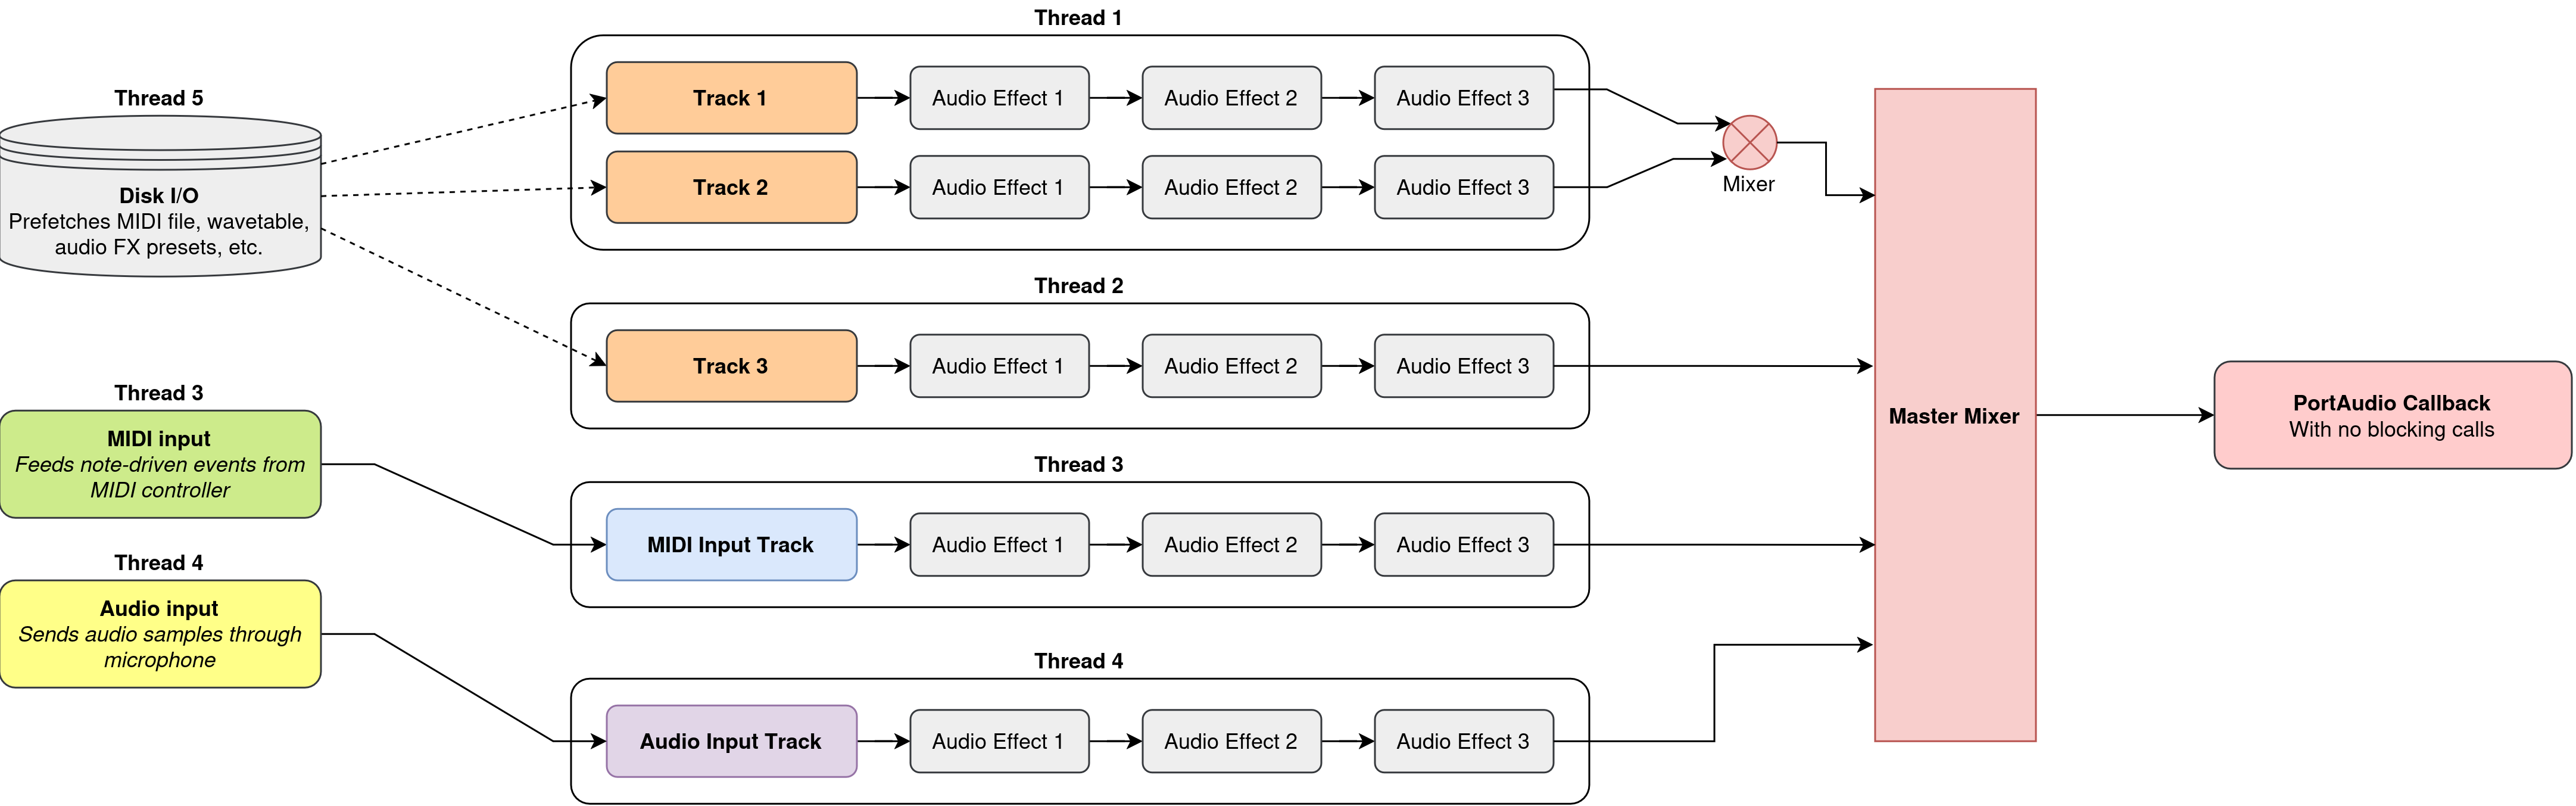
\includegraphics[width=\linewidth]{01_introduction/figures/architecture.png}
  \caption{Software Architecture of the DAW with Thread and Track Management}
  \label{fig:main_daw_architecture}
\end{figure}

Since the project is currently under construction, the actual 
stress test has not yet been performed due to limited number of components. But rather, an estimation
is conducted using a mockup DAW session containing only a list of instruments with no MIDI events,
and a look-up table containing measured execution times for each components. The Direct Acyclic Graph (DAG) 
technique \cite{susser_adc2025} is used to find the critical path, which is then used to calculate the overall 
execution time. This provides a reasonable amount of evidence to determine whether the tracks and audio effects 
would meet its deadline or not.
